\chapterimage{head2.png} % Chapter heading image
\chapter{Latex examples}

% ---------------------------------------------
% ---------------------------------------------
\section{Sample text}
So, as an engineer without any astrophysics background I thought I would be doing image processing applied to astronomy and I ended up doing so much more, but hey! You never know what you will end up doing.

Before coming to Canada, Pauline and I exchanged some emails where she shared me some interesting papers, web pages and an astronomy on-line course which later I did take, mainly the information was about a general introduction to astronomy and how astronomy images are, yes, astronomy images are completely different as any other \emph{normal} images, they are made of purely science data and every image has valuable knowledge you can learn from, and hey you will forget soon about pixels and start talking about sky coordinates.

So, in a few words I had no idea of what I was going to do (still), I realized I didn't have any idea, and the only thing I understood was how CCD detectors work. I didn't know I had a research adventure awaiting for me.

% ---------------------------------------------
% ---------------------------------------------
\section{Itemizes and enumerates}\index{Objective}
After I arrived and had my first meeting with Pauline, she explained me a general idea of what she wanted and shared me some more papers (about multi-wavelength studies), I read the information and came up with the objective.

\begin{itemize}
\item Find out a method to transform data from a high dimensional dataset (FITS cube or any other data arrangement) to a low dimensional understandable information (graphs, clusters).
\item Find out a method to transform data from a high dimensional dataset (FITS cube or any other data arrangement) to a low dimensional understandable information (graphs, clusters).
\end{itemize}

This means that from multiple images with different wavelengths of the same target apply an algorithm to find the hidden patterns that lie hidden between them.

% ---------------------------------------------
% ---------------------------------------------
\section{subsections}
OK, here is where I explain from where this is going to start, at that time I just had a micro-controllers and engineering design course my mind was set completely to find applicable theories and create useful things with them, which is the complete opposite of how astronomy works. First, there's no way to test an experiment with galaxies and most of the information is fuzzy and subjective (not all). The process of having an, let's say \emph{astronomy idea} is a result of applying all your physics knowledge and consider the \textbf{cosmological principle},

\subsection{Subsection example}
Since I found so much good information about pretty much everything I wanted to know about, I will just create a remark and let you know where you can find more specific information about, just like below.

\subsubsection{Subsubsection example}
Since I found so much good information about pretty much everything I wanted to know about, I will just create a remark and let you know where you can find more specific information about, just like below.

\subsubsection{Another subsubsection example}
Since I found so much good information about pretty much everything I wanted to know about, I will just create a remark and let you know where you can find more specific information about, just like below.

\subsection{Another subsection example}
Since I found so much good information about pretty much everything I wanted to know about, I will just create a remark and let you know where you can find more specific information about, just like below.

% ---------------------------------------------
% ---------------------------------------------
\section{References}
In \cite{book_key} authors talk about bla bla bla.

% ---------------------------------------------
% ---------------------------------------------
\section{Images}
Figure \ref{fig:nine} shows bla bla.

\begin{figure}
	\centering
    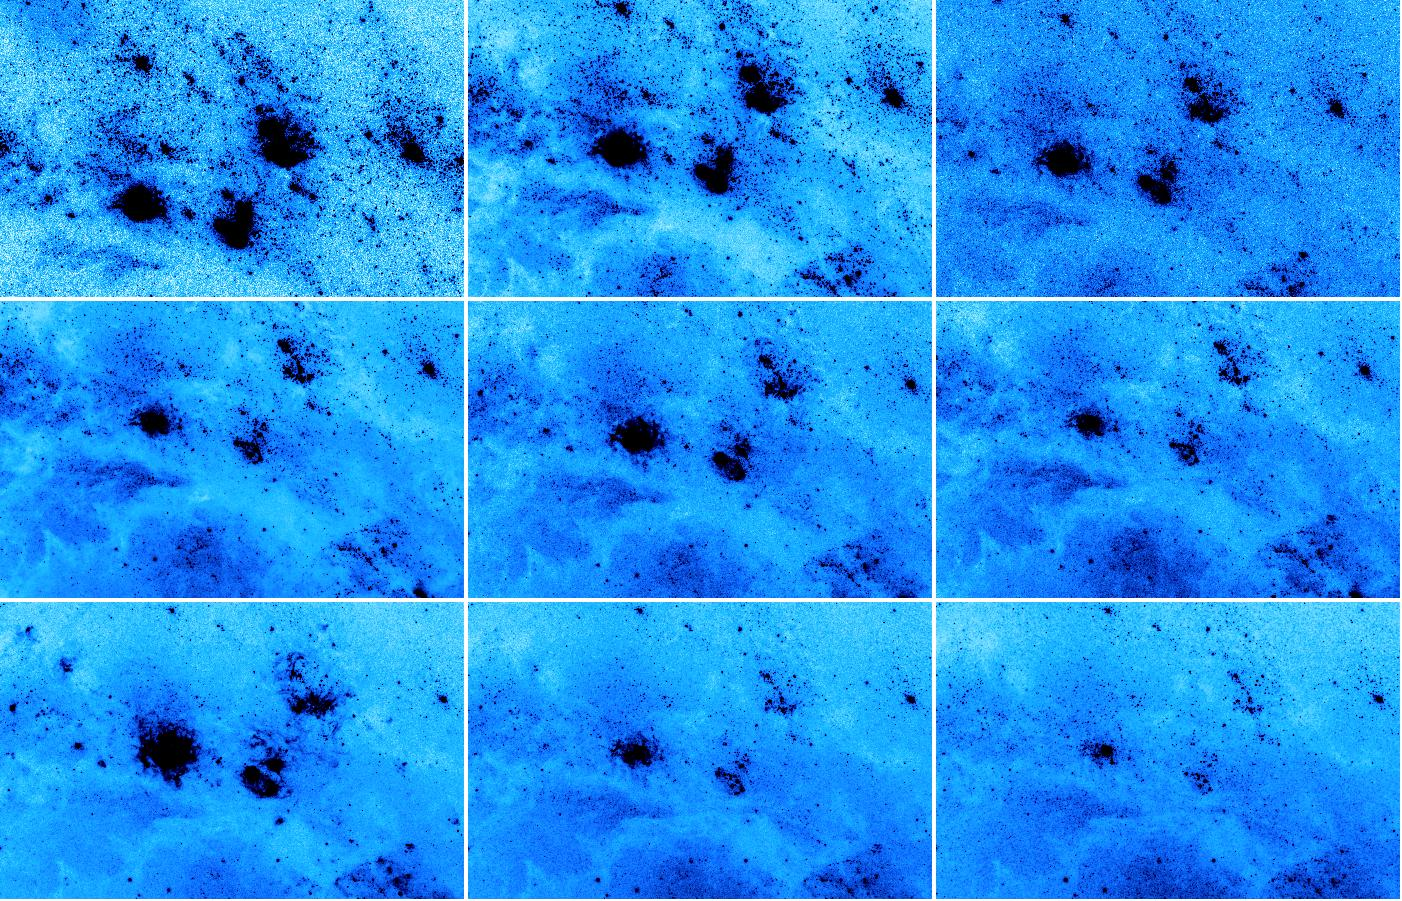
\includegraphics[width=0.87\textwidth]{nine.jpg}
    \caption{Example of how an object can look in 9 wavelengths}
    \label{fig:nine}
\end{figure}

% ---------------------------------------------
% ---------------------------------------------
\section{Tables}
Table \ref{tab:dos} shows bla bla bla.

\begin{table}[h]
    \centering
    \caption{WFC3/UVIS PSF FWHM informations for the selected dataset, as you can see the largest number here is 0.083 which means the poorest spatial resolution, this is the number used to calculate the convolution kernel, in order to precess them all images must have the same spatial resolution.}
    \label{tab:dos}
      \begin{tabular}{ c c c }
      \hline\hline
      
      Filter / Config. & Central $\lambda$ & FWHM (arc sec)\\
      \hline
      F225W & 235.9 nm & $\sim$0.083\\      
      F336W & 335.5 nm & $\sim$0.075\\      
      F373N & 373.0 nm & $\sim$0.070\\
      F438W & 432.5 nm & $\sim$0.070\\
      F487N & 487.1 nm & $\sim$0.067\\
      F502N & 501.0 nm & $\sim$0.067\\
      F657N & 656.7 nm & $\sim$0.070\\
      F673N & 676.6 nm & $\sim$0.070\\
      F814W & 802.4 nm & $\sim$0.074\\
      
      \hline
    \end{tabular}
  \end{table}
  

% ---------------------------------------------
% ---------------------------------------------
\section{Links}
\url{https://github.com/LaurethTeX/Clustering/blob/master/Tools.md#the-profile-file}


